% !TeX spellcheck = da_DK
\subsection{Accelerometer}
Accelerometeret ADXL335, som ses på \figref{ADXL335} er en treakset sensor, som kan anvendes til måling af statisk balance. Accelerometeret har en single-supply spændingsforsyning, der skal være mellem 1.8 - 3.6 V. På dette accelerometer er der tilkoblet en regulator, hvilket forhindre input-spænding over 3.3 V.  Arbejdsområdet ligger mellem $\pm$ 3.6 g og outputtet fra accelerometeret er maksimalt på $\pm$ 1.3 V. Båndbredden for X og Y-akserne ligger mellem 0.5 til 1600 Hz og for Z-aksen mellem 0.5 til 550 Hz. Støjen fra Xout og Yout ligger normalt på 150 $\mu g/\sqrt{Hz * rms}$, mens det for Zout ligger på 300 $\mu g/\sqrt{Hz * rms}$. Offsettet varierer efter spændingsforsyningen men ligger ved 3 V forsyning på 1500 mV og beregnes som $ Off = Vs/2$.  Sensitiviteten afhænger ligeledes af spændingsforsyningen, da accelerometeret er ratiometrisk og ligger ved 3 V forsyning mellem 270 og 330 mV/g. Output signalet er en analog spænding som er proportionel med accelerationen. %Outputtet ligger normalt ved -1.08g i X-aksen og  1.08g Y-aksen og 1.83 g ved Z-aksen. 

\begin{figure}[H]
\centering 
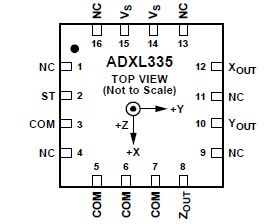
\includegraphics[scale=1]{figures/cProblemloesning/ADXL335.JPEG}
\caption{Accelerometeret ADXL335, hvor de forskellige indgange ses samt i hvilken retning akserne forløber}
\label{ADXL335}
\end{figure}

Når accelerometeret hældes til siden, vil der ske en acceleration ift. tyngdekraften i en given retning og dermed et udslag fra referencepunktet, som er ved en hældning på 0$^{\circ}$. Sammenhængen mellem de enkelte parametre kan udtrykkes ved følgende ligning:\\ 
\begin{equation}
$Vout=Voffset+sensitiviteten*tyngdekraften*sin(vinklen)$ \\
$Vout=Voffset+(\frac{\frac{\Delta V}{\Delta g} * g * \sin(\Theta))$
\end{equation}

Herudfra er det muligt at isolere og udregne de ukendte parametre, altså kan patientens hældningsgrad bestemmes ud fra accelerometerets output.

